%%%%%%%%%%%%%%%%%%%%%%%%%%%%%%%%%%%%%%%%%
% Arsclassica Article
% LaTeX Template
% Version 1.1 (10/6/14)
%
% This template has been downloaded from:
% http://www.LaTeXTemplates.com
%
% Original author:
% Lorenzo Pantieri (http://www.lorenzopantieri.net) with extensive modifications by:
% Vel (vel@latextemplates.com)
%
% License:
% CC BY-NC-SA 3.0 (http://creativecommons.org/licenses/by-nc-sa/3.0/)
%
%%%%%%%%%%%%%%%%%%%%%%%%%%%%%%%%%%%%%%%%%

%----------------------------------------------------------------------------------------
%    PACKAGES AND OTHER DOCUMENT CONFIGURATIONS
%----------------------------------------------------------------------------------------

\documentclass[
10pt, % Main document font size
a4paper, % Paper type, use 'letterpaper' for US Letter paper
oneside, % One page layout (no page indentation)
%twoside, % Two page layout (page indentation for binding and different headers)
headinclude,footinclude, % Extra spacing for the header and footer
BCOR5mm, % Binding correction
]{scrartcl}
\usepackage[]{algorithm2e}
\usepackage{framed}
\usepackage{listings}
\lstset{
  mathescape,
  columns=fullflexible,
  basicstyle=\fontfamily{lmvtt}\selectfont,
}


%%%%%%%%%%%%%%%%%%%%%%%%%%%%%%%%%%%%%%%%%
% Arsclassica Article
% Structure Specification File
%
% This file has been downloaded from:
% http://www.LaTeXTemplates.com
%
% Original author:
% Lorenzo Pantieri (http://www.lorenzopantieri.net) with extensive modifications by:
% Vel (vel@latextemplates.com)
%
% License:
% CC BY-NC-SA 3.0 (http://creativecommons.org/licenses/by-nc-sa/3.0/)
%
%%%%%%%%%%%%%%%%%%%%%%%%%%%%%%%%%%%%%%%%%

%----------------------------------------------------------------------------------------
%	REQUIRED PACKAGES
%----------------------------------------------------------------------------------------

\usepackage[
nochapters, % Turn off chapters since this is an article        
beramono, % Use the Bera Mono font for monospaced text (\texttt)
eulermath,% Use the Euler font for mathematics
pdfspacing, % Makes use of pdftex’ letter spacing capabilities via the microtype package
dottedtoc % Dotted lines leading to the page numbers in the table of contents
]{classicthesis} % The layout is based on the Classic Thesis style

\usepackage{arsclassica} % Modifies the Classic Thesis package

\usepackage[T1]{fontenc} % Use 8-bit encoding that has 256 glyphs

\usepackage[utf8]{inputenc} % Required for including letters with accents

\usepackage{graphicx} % Required for including images
\graphicspath{{Figures/}} % Set the default folder for images

\usepackage{enumitem} % Required for manipulating the whitespace between and within lists

\usepackage{lipsum} % Used for inserting dummy 'Lorem ipsum' text into the template

\usepackage{subfig} % Required for creating figures with multiple parts (subfigures)

\usepackage{amsmath,amssymb,amsthm} % For including math equations, theorems, symbols, etc

\usepackage{varioref} % More descriptive referencing

%----------------------------------------------------------------------------------------
%	THEOREM STYLES
%---------------------------------------------------------------------------------------

\theoremstyle{definition} % Define theorem styles here based on the definition style (used for definitions and examples)
\newtheorem{definition}{Definition}

\theoremstyle{plain} % Define theorem styles here based on the plain style (used for theorems, lemmas, propositions)
\newtheorem{theorem}{Theorem}

\theoremstyle{remark} % Define theorem styles here based on the remark style (used for remarks and notes)

%----------------------------------------------------------------------------------------
%	HYPERLINKS
%---------------------------------------------------------------------------------------

\hypersetup{
%draft, % Uncomment to remove all links (useful for printing in black and white)
colorlinks=true, breaklinks=true, bookmarks=true,bookmarksnumbered,
urlcolor=webbrown, linkcolor=RoyalBlue, citecolor=webgreen, % Link colors
pdftitle={}, % PDF title
pdfauthor={\textcopyright}, % PDF Author
pdfsubject={}, % PDF Subject
pdfkeywords={}, % PDF Keywords
pdfcreator={pdfLaTeX}, % PDF Creator
pdfproducer={LaTeX with hyperref and ClassicThesis} % PDF producer
} % Include the structure.tex file which specified the document structure and layout

\hyphenation{Fortran hy-phen-ation} % Specify custom hyphenation points in words with dashes where you would like hyphenation to occur, or alternatively, don't put any dashes in a word to stop hyphenation altogether

%----------------------------------------------------------------------------------------
%    TITLE AND AUTHOR(S)
%----------------------------------------------------------------------------------------

\title{\normalfont\spacedallcaps{White Paper}} % The article title

\author{\spacedlowsmallcaps{Sleepy Consensus Simulator}} % The article author(s) - author affiliations need to be specified in the AUTHOR AFFILIATIONS block

\date{\today} % An optional date to appear under the author(s)

%----------------------------------------------------------------------------------------

\begin{document}

%----------------------------------------------------------------------------------------
%    HEADERS
%----------------------------------------------------------------------------------------

\renewcommand{\sectionmark}[1]{\markright{\spacedlowsmallcaps{#1}}} % The header for all pages (oneside) or for even pages (twoside)
%\renewcommand{\subsectionmark}[1]{\markright{\thesubsection~#1}} % Uncomment when using the twoside option - this modifies the header on odd pages
\lehead{\mbox{\llap{\small\thepage\kern1em\color{halfgray} \vline}\color{halfgray}\hspace{0.5em}\rightmark\hfil}} % The header style

\pagestyle{scrheadings} % Enable the headers specified in this block

%----------------------------------------------------------------------------------------
%    TABLE OF CONTENTS & LISTS OF FIGURES AND TABLES
%----------------------------------------------------------------------------------------

\maketitle % Print the title/author/date block

\setcounter{tocdepth}{2} % Set the depth of the table of contents to show sections and subsections only

\tableofcontents % Print the table of contents
\newpage

%----------------------------------------------------------------------------------------

\newpage % Start the article content on the second page, remove this if you have a longer abstract that goes onto the second page

%----------------------------------------------------------------------------------------
%    Mission
%----------------------------------------------------------------------------------------

\section{Mission}
Implementation of a distributed consensus protocol in the sleepy model for pedagogical use. In the sleepy consensus protocol, we adopt a leader election to refrain from the computing resources' waste of the core idea behind Nakamoto's blockchain protocol\textemdash"proofs-of-work", with static corruption and synchronized clocks. The \textit{Adversary} could control all corrupted nodes and have the ability to delay messages up to $\Delta$ time. The corrupted nodes hack the blockchain network with selfish mining and consistency attack. Finally, we will see that without the majority of the honest nodes, the properties\textemdash\textit{consistency} and \textit{quality} of the blockchain can't be guaranteed.
%----------------------------------------------------------------------------------------
%    Our Team
%----------------------------------------------------------------------------------------

\section{Our Team}

\begin{table}[h]
    \centering
    \begin{tabular}{|c|c|c|c|c|}
        \hline
        Framework  & Lequn Chen & Bicheng Gao  & Songyu Ke  & Shichao Xu   \\ \hline
        Honest     & Wanquan Wu & Ziqi Zeng    & Yi Jiang   & Zhendong Xue \\ \hline
        Adversary  & Haoming Lu & Yuhao Zhou   & Xuan Zhang & Cheng Wan    \\ \hline
        Integrator & Zihao Ye   & Xueyuan Zhao & Yunqi Li   & Zhi Qiu      \\ \hline
    \end{tabular}
\end{table}
%----------------------------------------------------------------------------------------
%    Distributed Consensus
%----------------------------------------------------------------------------------------

\section{Distributed Consensus}

\subsection{Introduction}

First, we will talk about distributed consensus. In a distributed system, there are some rules that every node should follow. Honest nodes will behave according to those rules, while the corrupted nodes won't. Under the interference of corrupted nodes, we want all honest nodes to reach some kind of consensus. 

\subsubsection{Background}

The story starts from the Byzantine Generals' Problem. Byzantine is now located in Istanbul, Turkey, which is the capital of the Eastern Roman Empire. Because at that time the Byzantine Roman Empire was vast, for the purpose of defense, each army is very far apart. The generals can only rely on the message sent by postmen to communicate with each other. At the time of the war, all the generals in the Byzantine army should reach a consensus whether to attack or not. But there may have traitors in the arm. At this time, in the case of known members of the rebellion, the remaining loyal generals to reach a consensus agreement without the influence of the traitors is the key to this problem.\\ \\
In a distributed system, usually, our goal is to reach Byzantine Agreement. There may have some corrupted nodes controlled by the force of evil. Nodes exchange messages through the pairwise link. At the beginning, a sender node will send messages to other nodes. If the sender is honest, it will send the same message to everyone. Otherwise, things become more complicated. Later on, every node sends the message it received to its neighboring nodes.  Finally, we want all honest node to reach an agreement, which means all honest nodes have the same output. Moreover, if the sender is honest, then everyone outputs the message it received from the sender.

\subsubsection{Consensus}
Consensus protocols are the most critical research object of distributed computing. A dream consensus protocol will realize a "linearly ordered log" abstraction, which often referred to as \textit{state machine replication} in distributed systems literature. Simply speaking, every node maintains an ever-growing ordered log of transactions. The log should satisfy two properties:
\begin{itemize}
    \item \textbf{Consistency} \\
    At any time, all honest nodes have consistent logs(For any two honest nodes, either their logs are the same, or one log is the prefix of another). And each log should be self-consistent. 
    \item \textbf{Liveness} \\
    If some honest node receives a transaction \textit{tx} as input, or if \textit{tx} appears in some honest node's output log, then \textit{tx} will appear in every other participant's log within some fixed(small) amount of time.
\end{itemize}

\subsubsection{Permission and Permissionless}

Distributed systems have been analyzed historically in a permission setting. In this situation, everyone knows the number of the participants in the system. And the communication channels among nodes are authenticated.\\ \\ 
With the development of the peer-to-peer system, eventually, people transfer interest to the permissionless system. In this case, every node is uncurtained about the exact number of participants. Anyone can join the protocol execution without getting permission from a centralized or distributed authority. Moreover, the communication channels are unauthenticated.\\ \\
The difficulty of achieving permissionless consensus is the existence of so-called "Sybil attack", which can be easily implemented by spawning lots of nodes so it can control the majority of the nodes.
 

\subsection{Nakamoto’s Blockchain}
\subsubsection{Protocol Description}
  In Nakamoto's Blockchain model, every node maintains a $\mathsf{chain}$.
  When a node receives a $\mathsf{chain}$ that is valid, it will update the chain in the following way:
 \begin{lstlisting}
if $|\mathsf{chain'}| > |\mathsf{chain}|$:
    $\mathsf{chain} := \mathsf{chain'}$
    broadcast $\mathsf{chain}$
  \end{lstlisting}
\subsubsection{Proof of work}
In every round of an execution with security parameter $\mathcal{K}$, we assume all nodes have access to a random function $H:\{0 , 1\}    ^* \rightarrow \{0, 1\}^\mathcal{K}$. Let $TXs$ be the set of transactions in view but not appearing in $\mathsf{chain}[:-T]$.
\begin{lstlisting}
$\eta \leftarrow_{\$}\{0,1\}^{\kappa}$
if $H(\mathsf{chain}, \mathsf{TXs}, \eta) < D$:
    $\mathsf{chain} := \mathsf{chain} \ || \ (\mathsf{TXs}, \eta)$
    broadcast $\mathsf{chain}$
\end{lstlisting}

For our time stamp network, we implement the proof-of-work by incrementing $\eta$ in the block until a value is found that satisfies the corresponding hash function is less than a certain threshold $D$. 

\subsubsection{Security}
A blockchain protocol should satisfy chain growth, chain quality, and consistency. 

\begin{description}
\item[Chain growth]: Honest nodes' chains grow steadily, neither too fast nor too slow.

\item[Chain quality]: In any honest node's chain, any sufficiently long window of consecutive blocks contains a certain fraction of blocks that are mined by honest nodes.

\item[Consistency]
Except for $e^{-\Omega(T)}$ fraction of execution traces, let $\mathsf{chain}_i^r$, $\mathsf{chain}_j^{r'}$ denote honest node $i$ and $j$'s chains in round $r$ and $r'$ where $r'>r$, then $\mathsf{chain}_i^r[:-T] \prec \mathsf{chain}_j^{r'}$.

\end{description}

\subsubsection{Attack Methods}
    One famous adversarial algorithm is called \textit{selfish mining}, which means when a corrupt node mines a block, it doesn't release its private chain immediately. Instead, it withholds its private chain until it observes some honest node has mined a chain of the equal enough. Then it releases private chain ahead of honest nodes, wasting the mining power of honest nodes. 
%----------------------------------------------------------------------------------------
%    Sleepy Consensus
%----------------------------------------------------------------------------------------

\section{Sleepy Consensus}
\subsection{Problem Set}
Before we talk about the protocol, we firstly show the following assumptions:


\begin{description}
\item[Synchronized clocks]:
We assume that all nodes can access a globally synchronized clock that ticks over time. Each clock tick is referred as an atomic \textit{time step}. Nodes can perform unbounded polynomial amount of computation in each time step, as well as receive and send polynomially many messages.
\item[Public-key infrastructure]:
We assume that there exists a public-key infrastructure(PKI). More specifically, we shall assume that the PKI is an ideal functionality $F_{CA}$(only available to the current protocol instance) that does the following:
\begin{itemize}
    \item On receiving \verb|register(pk)| from $P$, remember the pair $($\verb|pk|$, P)$ and ignore any future message from $P$.
    \item On receiving \verb|lookup(|$P$\verb|)|: return the store \verb|pk| or $\perp$ if not found.
\end{itemize}
\item[Network delivery]:
The adversary controls the message delivery between nodes. We assume that the adversary can arbitrarily delay and reorder messages, as long as all the messages sent from honest nodes are received by all honest nodes within $\Delta$ time steps.
\item[Static Corruptions]:
We assume that once our protocol starts to run, the environment can not corrupt an honest node and the corrupt node can not become an honest node.
\end{description}

\subsection{Protocol Description}
In distributed computing, typically we consider two types of nodes\textemdash\textit{honest} nodes and \textit{corrupted} nodes. We implemented a distributed consensus protocol in the sleepy model, which assumes that a $majority$ of the nodes are honest. It significantly departs from key ideas behind Nakamoto's blockchain protocol\textemdash the need for "proofs-of-work". The protocol relies on Public-Key-Infrastructure(PKI) and all nodes are assumed to have synchronized clocks.
\par As showed by Pass and Shi \cite{cryptoeprint:2016:918}. One target of sleepy consensus protocol is to remove the proof-of-work from the Nakamoto blockchain while maintaining provable guarantees. To remove the proof-of-work from Nakamoto's protocol, we make the following changes: we define the puzzle solution to be the form of $(P, t)$ instead of rate limiting through computational power, where $P$ is the player's identifier and $t$ is the block-time. The pair $(P, t)$ is a "valid puzzle solution" if $H(P,t) < D_p$ where $H$ denotes a pseudorandom function with a common reference string and $D_p$ is a parameter such that the has outcome is only smaller than $D_p$ with probability $p$. If $H(P,t) < D_p$ we say that $P$ is \textit{elected leader at time t}. Note that several nodes may be elected leaders at the same time steps.
\par A node $P$ that is elected leader at time step $t$ can extend a chain with a block that includes the solution $(P, t)$, the previous block's hash $h_{-1}$ and the transactions $TXs$ to be confirmed. To verify that the block indeed came from $P$, we require that the entire contents of the block i.e. $(h_{-1}, TXs, t, P)$ are signed under $P$'s public key. The same as Nakamoto's protocol, each node chooses the longest valid chain it has ever seen and extends the longest chain.
\par Note that the honest node's only attempt to mine solutions of the form $(P, t)$, where $t$ is the current time step, however, the adversary may use incorrect block-times such as the time in the future or the time in the past. To prevent this kind of attacks from happening, we have the following additional restrictions on the block-times in a valid chain:
\begin{enumerate}
    \item A valid chain must have strictly increasing block-times;
    \item A valid chain cannot contain any block-times for the future;
\end{enumerate}
We present our Sleepy consensus protocol as follows:
\begin{itemize}
    \item On input \verb|init()| from environment $Z$: \\
        Generate \verb|(pk, sk)|, register \verb|pk| with $F_{CA}$, initialize
        \[chain := (\perp,\perp,time=0,\perp,\perp,h=0)\]
    \item On receive $chain'$: \\
        If $|chain'| > |chain|$ and $chain'$ is valid and $H(P,t) < D_p$ for valid $P$ and $t$, then $chain := chain'$ and broadcast $chain$.
    \item For every time step $t$ and every honest node with party $P$:
    \begin{itemize}
        \item Receive transactions $TXs$ from environment $Z$.
        \item If $H(P, t) < D_p$ then let:
        \[
            \delta := \verb|sign|(\verb|sk|, chain[-1].h, TXs, t)
        \]
        and
        \[
            h' := hash(chain[-1].h,)
        \]
        Then let
        \[
            chain := chain || (chain[-1].h, TXs, t, P, \delta, h')
        \]
        \item Output \verb|extract(|chain\verb|)| to $Z$, where extract \verb|extract| is the function outputs an ordered list containing the $TXs$ extracted from each block in $chain$.
    \end{itemize}
\end{itemize}
Our protocol takes parameter $p$ as input, where $p$ is the probability each node is elected leader in a single time step. All nodes will invoke \verb|init| function once it is spawned.
%----------------------------------------------------------------------------------------
%    Simulator Components
%----------------------------------------------------------------------------------------
\section{Simulator Components}
In this section, we first introduce the overall structure of the simulator, then we introduce the three components of our simulator: Framework, Honest Party and Adversary Party. The last part of this section is the API document.
\subsection{Framework}
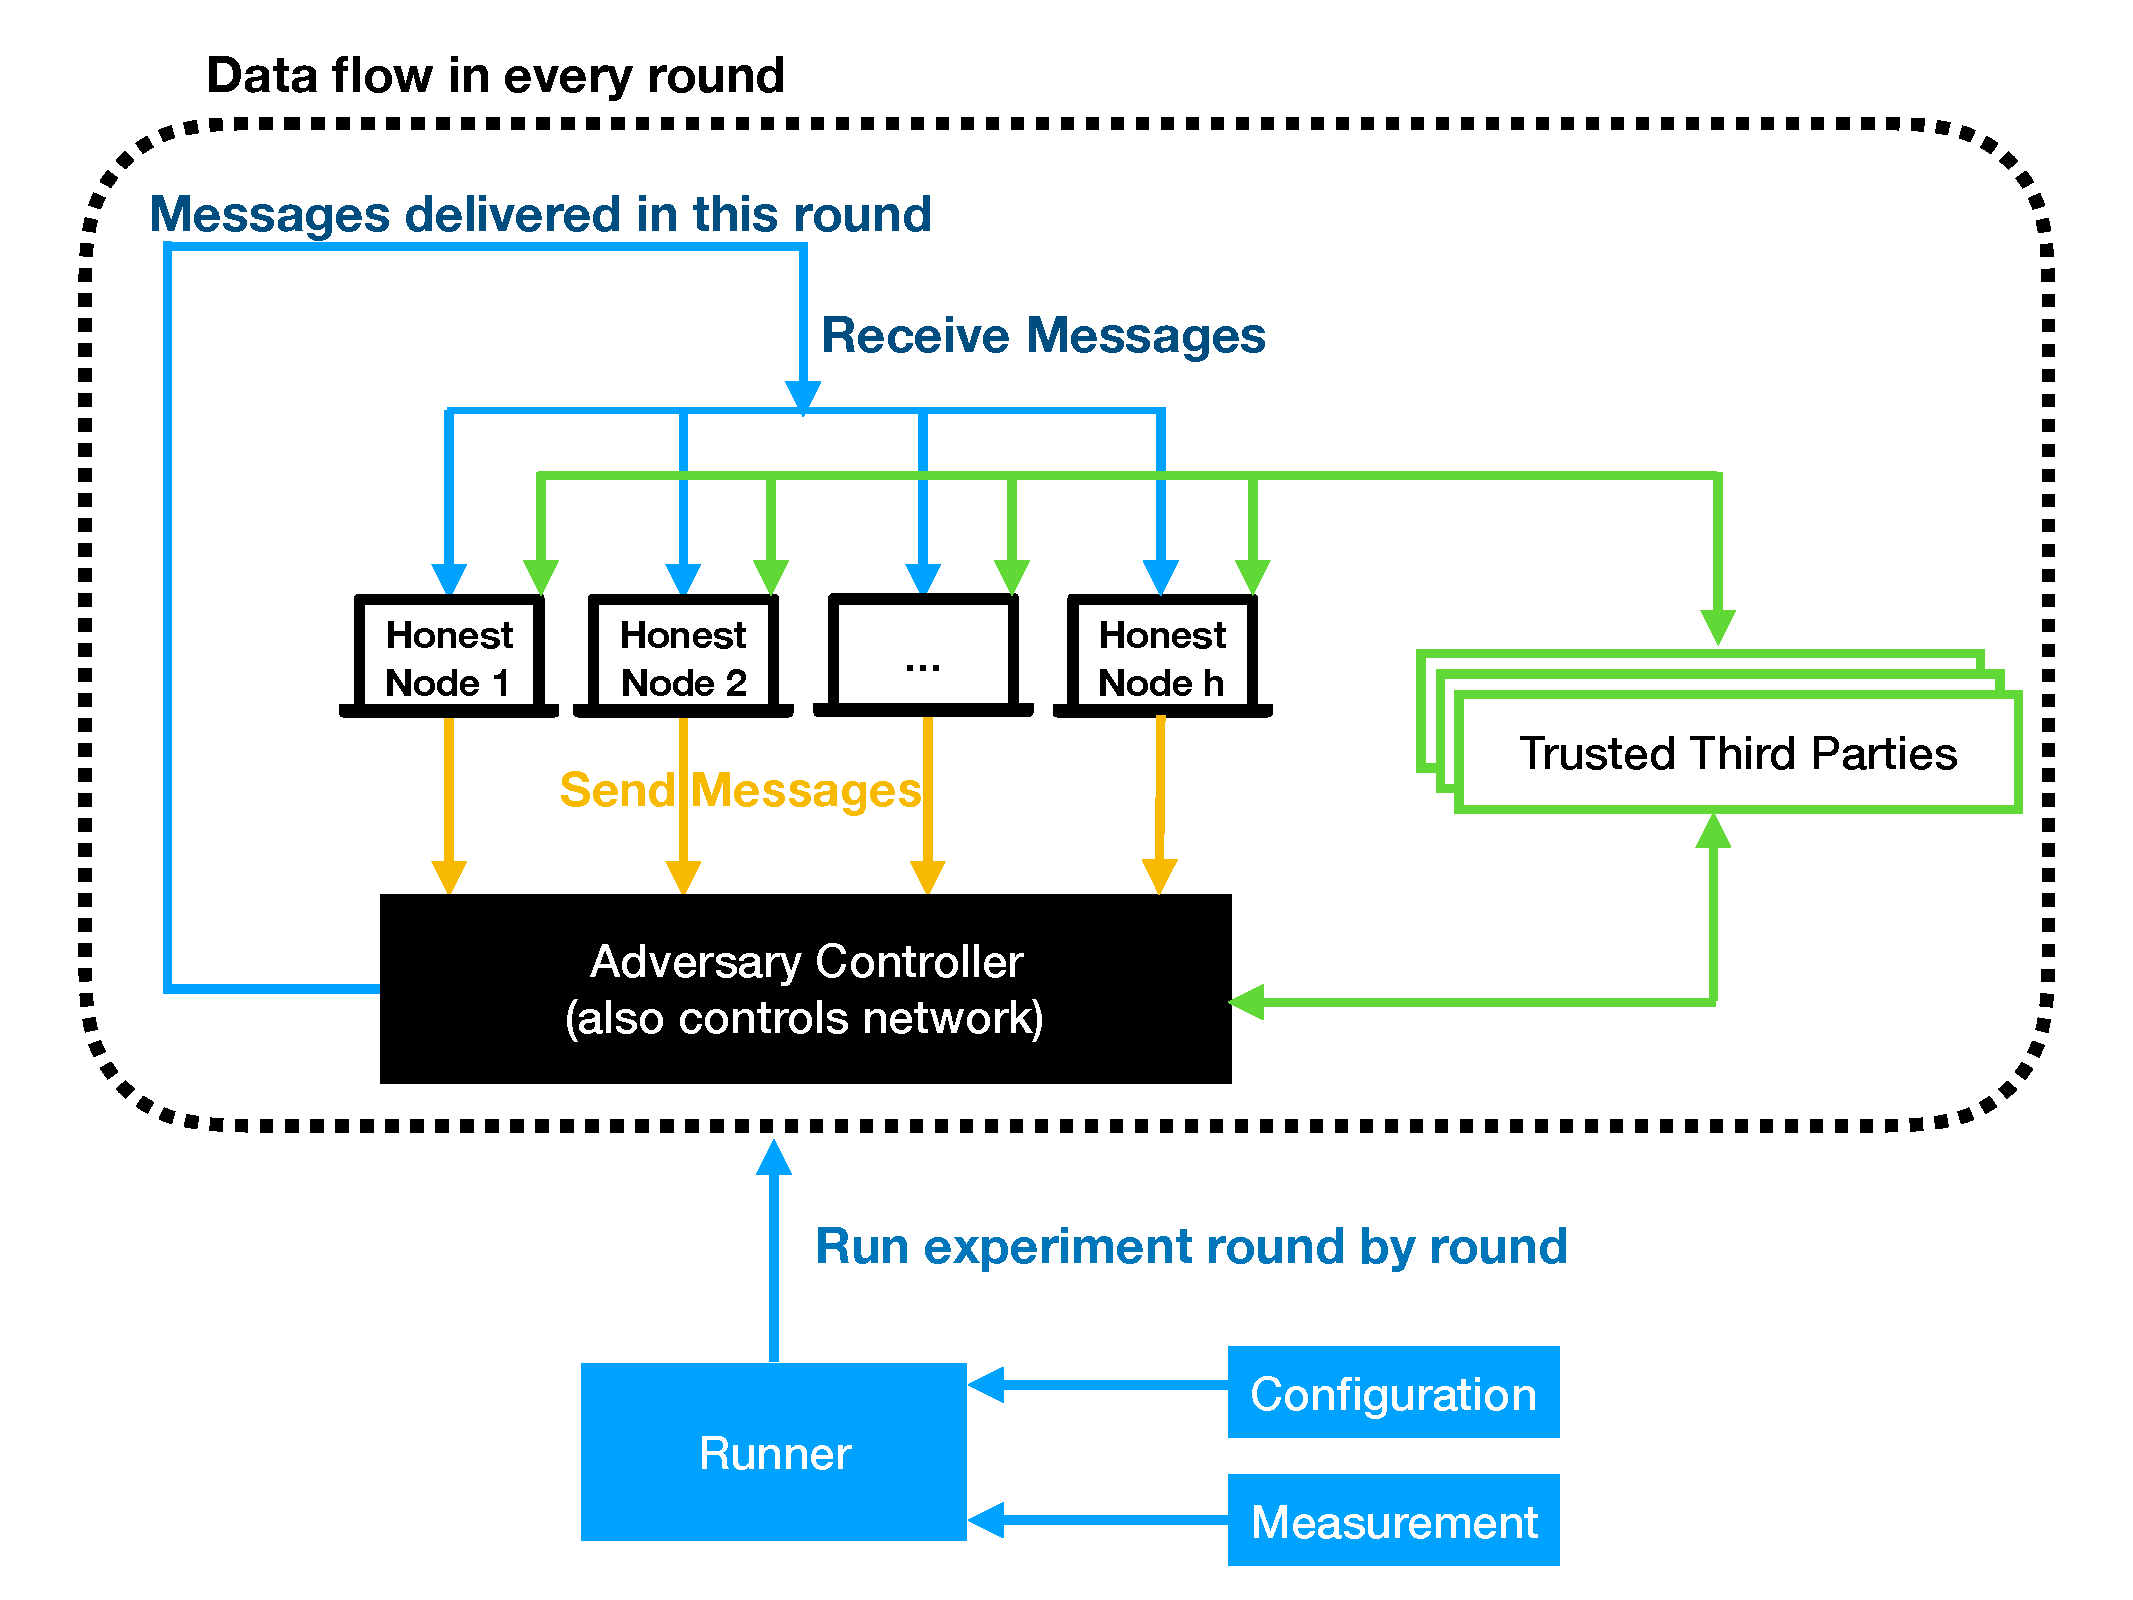
\includegraphics[scale=0.3]{structure}\\
As shown in the figure, our simulator runs in a round-by-round style. The class \verb|framework.Runner| controls the action in each round. By creating the subclasses of class \verb|framework.ConfigurationBase|, user can configure the parameters(e.g. number of rounds, ratio of corrupted nodes) the run. Users can write subclasses of the class \verb|framework.MeasurementBase| to provide the function of measuring the results(e.g. consistency and chain quality) of the experiment.
\par In each round, the adversary firstly delivers messages to the corresponding receivers. Then, the honest nodes send the messages to the adversary controller since the adversary has the control of the network. The class \verb|framework.Context| provides a easy way for the honest nodes to interact with the network.
\par The class \verb|utils.FSignRSA| and \verb|utils.FSignHash| plays the role of trusted third party. User can also create the subclasses of class \newline \verb|framework.TrustedThirdPartyBase|.

\subsection{Framework}
Our framework implement several abstract classes for the users implement their own subclasses:
\begin{itemize}
	\item class \verb|AdversaryControllerBase| is the super class for the user defined adversary party.
	\item class \verb|ConfigurationBase| is the super class for the user defined running configuration.
	\item class \verb|Context| the network interface for the nodes to communicate with each other.
	\item class \verb|MeasurementBase| is the super class for the user defined measurement.
	\item class \verb|NodeBase| is the super class for the user defined node type.
	\item class \verb|Runner| is the default round-by-round runner.
	\item class \verb|TrustedThirdPartyBase| is the super class for the user defined trusted third party. 
\end{itemize}
\subsection{Honest Party}
Each honest nodes has:
\begin{itemize}
\item node ID
\item \textbf{blockchain} Since blockchain will fork, it's actually a block tree. The longest chain is the main chain. According to Sleepy Consensus Protocol, the previous block should have smaller timestamp than the successor.
\item \textbf{transaction pool}\\
Receive transactions(\textit{tx}) from network and store in \textit{tx} pool temporarily. If the node receives a \textit{tx} not in current \textit{tx} pool, the node will forward(broadcast) this \textit{tx} with its own signature immediately. At the end of each round, all \textit{tx}s remained in \textit{tx} pool will form a new block append at the end of mainchain. 
\item    \textbf{orphan pool}\\ 
The node will receive blocks from the network. With the interference of \textit{Adv}, some blocks will be delayed, but not lost. Perhaps some successive blocks have already received, but they can't be connected to the block tree since they are waiting for their "father" block. So we need a "pool" to store those "orphan" block.\\
The delete operation of a block in the orphan pool is very tricky. We only store single blocks, but we need to remove all successors of it at the same time, which results to a recursive process. 

\item \textbf{probability}\\
\textit{probability} is related to the mining difficulty $D$. For node $x$, if the hash value of its node ID and the current time is less than $D$, then $x$ is elected as the leader who has the right to mine a new block and broadcast to other nodes.
\end{itemize}

\subsection{Adversary Party}
We implement 2 kinds of adversaries in this project: \textit{Selfish Mining Attack} and \textit{Consistency Attack}.
\subsubsection{Selfish Mining Attack}
Ittay Eyal and Emin Gun Sirer\cite{DBLP:journals/corr/EyalS13} introduced the selfish mining attack, and Buterin presented the adversary's precise strategy \href{https://bitcoinmagazine.com/articles/selfish-mining-a-25-attack-against-the-bitcoin-network-1383578440/}{here}. In our project, we implement this attack method as \verb|sleepy.SelfishMining| class and the corresponding measurement \verb|sleepy.ChainQualityMeasurement| class.
\subsection{Consistency Attack}
We also implemented a naive consistency attack which is described as follows:
\begin{itemize}
	\item Pick the longest chain from all honest chains and its private chain.
	\item For every honest message: delay by $\Delta$.
	\item If adversary’s private chain is longer than the honest chain and it's length is at least $T + 1$, then it publish the chain and will break consistency.
	\item Here $T$ is the security parameter, except with probability $e^{-\Omega(T)}$: \\
	$\forall$ honest chains $chain^{r}_{i}$ and $chain_{j}^{r'}$ s.t. $r' \geq r$, $chain_{i}^r[:\text{-T}] < chain_j^{r'}$
	\item When the adversary has 60\% of the computational power, he can keep developing his own private chain until honest chain is long enough, then release the chain to overwrite the last $ T $ blocks. So that the honest chain may be overwrite.
\end{itemize}
This attack method implemented in the class of \verb|sleepy.ConsistencyAttack|.
\subsection{API document}
\href{https://abcdabcd987.github.io/distributed-consensus-simulator/api_doc.html}{Here} is the link to the API document as well as the html version of this report.


%----------------------------------------------------------------------------------------
%    Experiment Results
%----------------------------------------------------------------------------------------
\section{Experiment Results}
For the 2 attacking methods, we implement several experiments on various sets of parameters. The following figure shows the relation between the probability of success and ratio of corrupted nodes for the naive consistency attack and the relation between chain quality between the ratio of corrupted nodes under the parameter setting of 
\[
	n=20,\Delta = 2, T = 6, p = 0.05
\]
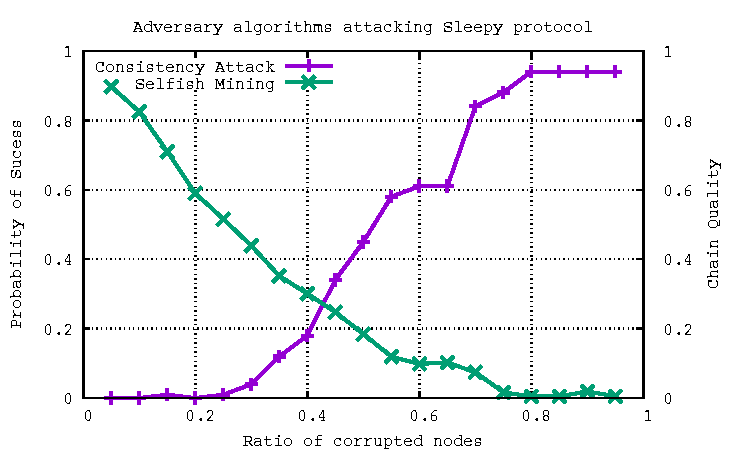
\includegraphics{Figures/results}
%----------------------------------------------------------------------------------------
%    BIBLIOGRAPHY
%----------------------------------------------------------------------------------------

\renewcommand{\refname}{\spacedlowsmallcaps{References}} % For modifying the bibliography heading

\bibliographystyle{unsrt}

\bibliography{sample.bib} % The file containing the bibliography

%----------------------------------------------------------------------------------------

\end{document}or modifying the bibliography heading

\bibliographystyle{unsrt}

\bibliography{sample.bib} % The file containing the bibliography

%----------------------------------------------------------------------------------------

\end{document}